 
    \section[The Problem of Nonobservability of  Interference and its Solution]{The Problem of Nonobservability of  Interference and its Solution\protect\footnotemark}\label{Nonobservability}\footnotetext{See \cite[55-57, 63-65]{Schlosshauer}. }Before we consider the many-worlds interpretation in detail, it will be helpful to consider the role that decoherence plays in the removal of quantum interference at the macroscopic scale, as it is this lack of quantum  interference between mutually exclusive states that justifies our belief that a system is in a definite state rather than in a superposition of alternative realities. The question of why quantum interference typically disappears at macroscopic scales is referred to as the problem of the nonobservability of interference. 
    
    We can explain this problem in the context of the double slit experiment:
    \begin{figure}[ht!]
    \captionsetup{justification=justified}
    \centering
    \begin{tikzpicture}
    \node[inner sep=0pt] (interfere) at (0,0)
     {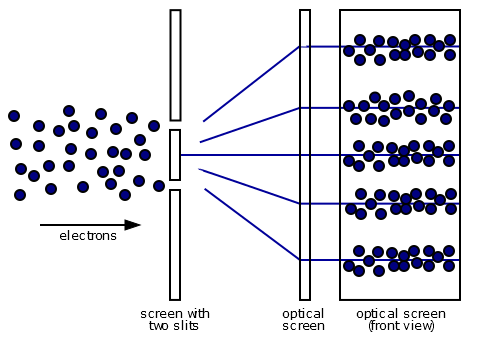
\includegraphics[width=.45\textwidth]{Chapter02/Two-Slit_Experiment_Electrons.png}}  ;
     \node[below right] at (interfere.south west) {(A) Particles exhibiting interference.};
     \node[inner sep=0pt] (noninterfere) at (7,0)
     {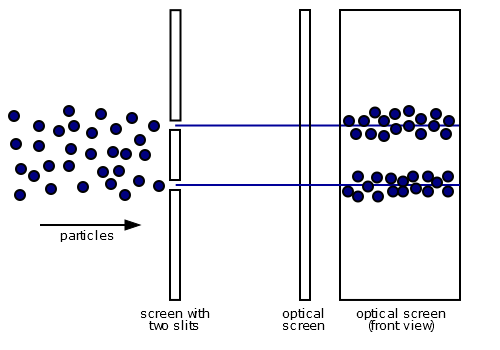
\includegraphics[width=.45\textwidth]{Chapter02/Two-Slit_Experiment_Particles.png}};
     \node[below right] at (noninterfere.south west) {(B) Particles not exhibiting interference.};
    \end{tikzpicture}
    \vspace*{10px}
    \caption[Double-Slit Experiment]{The Double-Slit Experiment. Particles are incident on a double slit. In diagram (A), the particles are exhibiting an interference pattern, whereas in diagram (B), the particles are not exhibiting an interference pattern. Whether or not there is interference will depend on factors such as the size of the particles and whether it can be ascertained which slit the particle went through. The larger the particles are, or the more information available as to which slit the particle went through, the less likely the particles will exhibit interference.\protect\footnotemark}
    \label{DoubleSlit}
    \end{figure}
    As figure \ref{DoubleSlit} indicates, when a beam of particles is incident on a double slit, the particles that are detected on the detection screen are distributed according to a distribution pattern which either exhibits quantum interference as shown on the left in the figure, or does not exhibit such interference as shown on the right. Small particles like electrons and photons will tend to exhibit quantum interference, whereas mesoscopic particles  will not typically exhibit quantum interference.\footnote{There are exceptions to this rule. For example, a \textbf{Superconducting Quantum Interference Devices (SQUID)}\index{Superconducting Quantum Interference Devices (SQUID)}  can demonstrate quantum interference even at macroscopic scales where a large superconductor can enter into a superposition of two states with the current flowing in opposite directions in each state. See \cite[ch. 6]{Schlosshauer}.}  
    
    To explain what is going on, we suppose that when just the top slit is open, the normalized state of the particle is $\ket*{\psi_1}$,\label{psi_slit} whereas if just the bottom slit is open, we suppose that the normalized state of the particle is $\ket*{\psi_2}$, and when both slits are open, we suppose that the state of the particle will be $\frac{1}{\sqrt{2}}(\ket*{\psi_1}+\ket*{\psi_2})$. 
     Now let the variable $x$ describe the position on the detection screen. For instance, we might take $x=0$ to be the center of the detection screen, and take  positive values of $x$ as corresponding to positions on the upper part of the screen, and negative values of $x$ as corresponding to positions on the lower part of the screen, but the precise convention we adopt won't matter.\footnotetext{Diagrams (A) and (B) are by inductiveload, and are Public domain, via Wikimedia Commons. Sources: https://commons.wikimedia.org/wiki/File:Two-Slit\_Experiment\_Electrons.svg and https://commons.wikimedia.org/wiki/File:Two-Slit\_Experiment\_Particles.svg.} Then we define the  $\ket*{x}$-state\footnotemark\;as the physical state describing the particle to be exactly located at position $x$ on the screen. Note that the state $\ket*{x}$ is indexed by a continuous parameter, $x$. This is in contrast to the basis of states $\ket*{s_i}$ which we have been considering up until now which are indexed by discrete values of $i$ such as $i=1,\,2,\ldots.$ Because of this difference, we need to use calculus to deal with $\ket*{x}$-states in a rigorous manner, but such details will not concern us here. In reality, because of the Heisenberg uncertainty principle, a particle is never in just one $\ket*{x}$-state, but rather the particle will be in a superposition of many $\ket*{x}$-states, which may or may not be concentrated around a particular location, $x_0$ say. The more concentrated these  $\ket*{x}$-states of this superposition are concentrated around a particular location $x_0$, the more the particle will have the particle-like characteristic of being localized in one place. But if the  $\ket*{x}$-states of this superposition are more spread out, the particle will have more wave-like characteristics. So when physicists speak of particles, often they are not thinking of physical entities that are very localized in position, as non-physicists would think. Nevertheless, at the moment the particle is detected on the detection screen, it does seem to be highly localized.\footnotetext{\label{ketx}$\ket*{x}$ is not really a state in the proper sense. With the states we've seen so far, when $\ket*{\phi}$ and $\ket*{\psi}$ have been normalized, then $\abs{\ip{\phi}{\psi}}^2$ will be a conditional probability, and hence at most $1$. However, $\ket*{x}$ %
\nomenclature{$\ket*{x}$}{A non-normalizable position state \nomrefpage}%
cannot be normalized. This is because the bracket  $\ip{x}{y}$ is defined to be $\ip{x}{y}=\var(x-y)$ where $\var(x)$ is the %
\nomenclature{$\var(x)$}{The Dirac delta function, \nomrefpage}%
     \emph{Dirac delta}\index{Dirac delta} function such that \begin{equation} 
    \var(x)=
    \begin{cases} \infty & \text{if $x=0$,} \\
    0 & \text{if $x\neq 0$},
    \end{cases}
    \end{equation} and has the property that 
    $\int \dd x \var(x) f(x) = f(0)$ for any continuous function $f(x)$. The theory of distributions allows one to deal rigorously with Dirac delta functions. E.g. see \cite[ch. 6]{Rudin}.  
    }
    
     Given a state $\ket*{\psi}$ for a so-called particle, we define the function $\psi(x)=\ip{x}{\psi}$.  %
\nomenclature{$\psi(x)$}{The wave function corresponding to the state $\ket*{\psi}$ given by the formula $\psi(x)=\ip{x}{\psi}$,  \nomrefpage}%
     Because of the continuous nature of the variable $x$ (in contrast to the discrete nature of $i$ in a basis $\{\ket*{s_i}:i\}$), the function 
     \begin{equation}\label{rhodensity}
     \rho(x)=\abs{\psi(x)}^2
     \end{equation} 
     determines a probability density for a range of outcomes rather than a probability for a specific outcome. Here, we do not need to go into the details of probability densities,\footnote{But if you are interested, a probability density $\rho(x)$ for a random variable $X$ that has real values is a function such that $\rho(x)\geq 0\, \,\forall x\in\mathbb{R}$, and that $\int_\mathbb{R} \rho(x) \dd x =1$ and the probability that $X$ has a value in the subset $U\subset\mathbb{R}$ is $\int_U \rho(x) \dd x $. } but roughly speaking, the greater the value of $\rho(x)$, the greater will be the relative probability of detecting the particle in the vicinity of location $x$. Thus, if $\rho(x')=0$ for all $x'$ in the vicinity of $x$, then the particle would not be detected in the vicinity of location $x$. 
    
    Now if  $\ket*{\psi}=\frac{1}{\sqrt{2}}(\ket*{\psi_1}+\ket*{\psi_2})$, then 
    $\psi(x)=\frac{1}{\sqrt{2}}(\psi_1(x)+\psi_2(x)).$ Therefore, the corresponding probability density will be
    \begin{equation*}\abs{\psi(x)}^2=\frac{1}{2}(\abs{\psi_1(x)}^2+\abs{\psi_2(x)}^2+2\Re(\overline{\psi_1(x)}\psi_2(x)).\protect\footnotemark
    \end{equation*}
    \footnotetext{Here $\Re$ %
\nomenclature{$\Re(z)$}{The real part of a complex number $z$,  \nomrefpage}%
    means the real part of a complex number. Thus, if the complex number $z=\alpha+i\beta$ for real numbers $\alpha$ and $\beta$, then $\Re(z)=\alpha$. To see why the above equation holds, we recall that $\abs{z}^2=z\overline{z}$ and that $\Re(z)=\frac{1}{2}(z+\overline{z})$. Therefore, if $z=\frac{1}{\sqrt{2}}(v+w)$ for complex number $v$ and $w$, then $\abs{z }^2 =\frac{1}{\sqrt{2}}(v+w)\frac{1}{\sqrt{2}}\overline{(v+w)}= \frac{1}{2}(v+w)\overline{(v+w)}=\frac{1}{2}(v\overline{v}+w\overline{w}+w\overline{v}+v\overline{w})=\frac{1}{2}(\abs{v}^2+\abs{w}^2+w\overline{v}+\overline{w\overline{v}})=\frac{1}{2}(\abs{v}^2+\abs{w}^2+2\Re(\overline{v}w))$.}Now when the detection screen is far away from the double slits, we will have $\abs{\psi_1(x)}^2\approx \abs{\psi_2(x)}^2$ for $x$ near the center point on the screen. However, depending on slight changes in the value of $x$ from the center point on the screen, sometimes $\psi_1(x)$ and $\psi_2(x)$ will be in phase so that  $\psi_1(x)\approx\psi_2(x)$, in which case $\abs{\psi(x)}^2\approx 2\abs{\psi_1(x)}^2$. But sometimes $\psi_1(x)$ and $\psi_2(x)$ will be  out of phase so that $\psi_1(x)\approx-\psi_2(x),$ in which case $\abs{\psi(x)}^2\approx 0$. Hence, we get the interference pattern as shown in figure \ref{DoubleSlit} (A).
    
    Now in order to consider how decoherence affects interference, we let $$\ket*{\Psi(t)}=\frac{1}{\sqrt{2}}(\ket*{\psi_1}\ket*{E_1(t)}+\ket*{\psi_2}\ket*{E_2(t)})$$ be the state of the composite system $\mathcal{U}=\mathcal{S}+\mathcal{E}$ where $\mathcal{S}$ is a particle that has gone through the double slit and will be detected on the detection screen, and $\mathcal{E}$ is the local environment of the experimental set up. The expression for $\ket*{\Psi(t)}$ indicates that we are assuming  $\mathcal{S}$ doesn't become entangled with $\mathcal{E}$ when $\mathcal{S}$ is in the state $\ket*{\psi_1}$ or $\ket*{\psi_2}$. Corresponding to $\ket*{\Psi(t)}$, we can define the density matrix  $\hat{\rho}(t)=\dyad{\Psi(t)}.$  We can also define the observable\footnote{Note that we only call $\dyad{x}_\mathcal{S}$ an observable in an analogical sense since it is not a compact Hermitian operator acting on the Hilbert space of states $H_\mathcal{S}$. If we were being more rigorous, we would need to consider a Hermitian operator of the form $\int \sigma(x)\dyad{x}_\mathcal{S}\dd x$ for an appropriate test function $\sigma(x)$. } $\dyad{x}_\mathcal{S}$ for the system $\mathcal{S}$ so that $\dyad{x}_\mathcal{S}\ket*{\psi}_\mathcal{S}=\psi(x)\ket*{x}_\mathcal{S}.$ As we saw in equation (\ref{extension}) on page \pageref{extension}, we can naturally extend the action of $\dyad{x}_\mathcal{S}$ to $H_\mathcal{U}$.\footnote{Strictly speaking, it is not $\dyad{x}_\mathcal{S}$ that is extended to act on $H_\mathcal{U}$, but rather a Hermitian operator of the form $\int \sigma(x)\dyad{x}_\mathcal{S}\dd x$ for an appropriate test function $\sigma(x)$ that is extended to $H_\mathcal{U}$. For a state $\ket*{\xi}_\mathcal{U}=\ket*{\psi}_\mathcal{S}\ket*{E}_\mathcal{E}$, the action of $\dyad{x}_\mathcal{U}$ on $\ket*{\xi}_\mathcal{U}$ gives the `state' $\dyad{x}_\mathcal{U}\ket*{\xi}_\mathcal{U}\myeq\psi(x)\ket*{x}_\mathcal{S}\ket*{E}_\mathcal{E}$, but since this is not normalizable, we have to `smear' it by integrating it with respect to the test function $\sigma(x)$.}  
    This allows us to define 
    $$\rho_\mathcal{U}(x, t)\myeq\Tr_\mathcal{U}(\hat{\rho}(t)_\mathcal{U}\dyad{x}_\mathcal{U}).$$
     In the specific case when $\mathcal{S}$ and $\mathcal{E}$ are not entangled so that $\hat{\rho}_\mathcal{U}(t)=\dyad{\xi(t)}_\mathcal{U}$ with $\ket*{\xi(t)}_\mathcal{U}=\ket*{\psi}_\mathcal{S}\ket*{E(t)}_\mathcal{E}$ for normalized states $\ket*{\psi}_\mathcal{S}$ and $\ket*{E(t)}_\mathcal{E}$, we have $\rho_\mathcal{U}(x, t) =\abs{\psi(x)}^2$ which is equal to the probability density function $\rho(x)$ we saw in equation (\ref{rhodensity}).\footnote{To see this, note that we can ignore $\mathcal{E}$ in calculating $\ev*{\dyad{x}_\mathcal{U}}_\xi$ since when $\mathcal{S}$ and $\mathcal{E}$ are not entangled, $\ev*{\dyad{x}_\mathcal{U}}_\xi = \ev*{\dyad{x}_\mathcal{S}}_\psi$ as explained in footnote \footreference{untangledobservable}. We can therefore just consider $\mathcal{S}$ and drop the subscripts.
    Furthermore, as we saw in equation (\ref{expdensity}), $\ev*{\hat{O}}_\psi=\Tr(\hat{\rho}\hat{O})$ where $\hat{\rho}=\dyad{\psi}$. 
    We can thus take an orthonormal basis $\{\ket*{\psi_1},\ket*{\psi_2},\ldots\}$ of $H_\mathcal{S}$ with $\ket*{\psi_1}=\ket*{\psi}$. 
    Then $\rho(x)=\Tr(\hat{\rho}\dyad{x})=\Tr(\dyad{\psi}\dyad{x})=\sum_i\ip{\psi_i}{\psi}\ip{\psi}{x}\ip{x}{\psi_i}=\ip{\psi_1}{\psi}\ip{\psi}{x}\ip{x}{\psi_1} =\ip{\psi}{x}\ip{x}{\psi}=\overline{\ip{x}{\psi}}\ip{x}{\psi}=\abs{\ip{x}{\psi}}^2=\abs{\psi(x)}^2.$} 
    However, if $\ket*{E_1(t)}_\mathcal{E}$ is not proportional to $\ket*{E_2(t)}_\mathcal{E}$, then $\ket*{\Psi(t)}$ will be an entangled state of $\mathcal{S}$ and $\mathcal{E}$. But whether or not $\mathcal{S}$ and $\mathcal{E}$ are entangled, we can still use equation (\ref{reduced}) to calculate the partial trace:
    $$\hat{\rho}_\mathcal{S}(t)=\frac{1}{2}(\dyad{\psi_1}_\mathcal{S}+\dyad{\psi_2}_\mathcal{S}+\ip{E_2(t)}{E_1(t)}_\mathcal{E} \dyad{\psi_1}{\psi_2}_\mathcal{S}+\ip{E_1(t)}{E_2(t)}_\mathcal{E} \dyad{\psi_2}{\psi_1}_\mathcal{S}).$$
    By equations (\ref{expdensity}) and (\ref{reducedev}), we therefore have
    \begin{equation}\rho_\mathcal{U}(x, t)=\frac{1}{2}\Big(\abs{\psi_1(x)}^2+\abs{\psi_2(x)}^2+2\Re\big(\ip{E_2(t)}{E_1(t)}_\mathcal{E}\overline{\psi_2(x)}\psi_1(x)\big)\Big).\protect\footnotemark
    \end{equation}
    Thus, \footnotetext{The calculation is as follows:
      \begin{equation*}
    \begin{split}\rho_\mathcal{U}(x, t)&=\Tr_\mathcal{U}(\hat{\rho}(t)_\mathcal{U}\dyad{x}_\mathcal{U})=
    \ev*{\dyad{x}_\mathcal{U}}_{\rho(t)}=\Tr_\mathcal{S}(\hat{\rho}_\mathcal{S}(t)\dyad{x}_\mathcal{S})\\
    &=\Tr_\mathcal{S}\Big(\frac{1}{2}(\dyad{\psi_1}_\mathcal{S}+\dyad{\psi_2}_\mathcal{S}\\
    &\qquad+\ip{E_2(t)}{E_1(t)}_\mathcal{E} \dyad{\psi_1}{\psi_2}_\mathcal{S}+\ip{E_1(t)}{E_2(t)}_\mathcal{E} \dyad{\psi_2}{\psi_1}_\mathcal{S})\dyad{x}_\mathcal{S}\Big)\\
    &=\Tr_\mathcal{S}\Big(\frac{1}{2}(\ip{\psi_1}{x}_\mathcal{S}\dyad{\psi_1}{x}_\mathcal{S}+\ip{\psi_2}{x}_\mathcal{S}\dyad{\psi_2}{x}_\mathcal{S}\\&\qquad+\ip{E_2(t)}{E_1(t)}_\mathcal{E}\ip{\psi_2}{x}_\mathcal{S}\dyad{\psi_1}{x}_\mathcal{S}+\ip{E_1(t)}{E_2(t)}_\mathcal{E} \ip{\psi_1}{x}_\mathcal{S}\dyad{\psi_2}{x}_\mathcal{S})\Big)
    \\
    &=\frac{1}{2}\Big(\ip{\psi_1}{x}_\mathcal{S}\ip{x}{\psi_1}_\mathcal{S}+\ip{\psi_2}{x}_\mathcal{S}\ip{x}{\psi_2}_\mathcal{S}\\&\qquad+\ip{E_2(t)}{E_1(t)}_\mathcal{E}\ip{\psi_2}{x}_\mathcal{S}\ip{x}{\psi_1}_\mathcal{S}+\ip{E_1(t)}{E_2(t)}_\mathcal{E}\ip{\psi_1}{x}_\mathcal{S}\ip{x}{\psi_2}_\mathcal{S}\Big)\\
    &=\frac{1}{2}\Big(\overline{\ip{x}{\psi_1}_\mathcal{S}}\ip{x}{\psi_1}_\mathcal{S}+\overline{\ip{x}{\psi_2}_\mathcal{S}}\ip{x}{\psi_2}_\mathcal{S}\\&\qquad+\ip{E_2(t)}{E_1(t)}_\mathcal{E}\overline{\ip{x}{\psi_2}_\mathcal{S}}\ip{x}{\psi_1}_\mathcal{S}+\overline{\ip{E_2(t)}{E_1(t)}_\mathcal{E}\overline{\ip{x}{\psi_2}_\mathcal{S}}\ip{x}{\psi_1}_\mathcal{S}}\Big)
    \\
    &=\frac{1}{2}\Big(\abs{\psi_1(x)}^2+\abs{\psi_2(x)}^2+2\Re\big(\ip{E_2(t)}{E_1(t)}_\mathcal{E}\overline{\psi_2(x)}\psi_1(x)\big)\Big).
    \end{split}
    \end{equation*}}if $\ip{E_1(t)}{E_2(t)}_\mathcal{E}\approx 0$ then 
    $\rho_\mathcal{U}(x, t)\approx\frac{1}{2}\Big(\abs{\psi_1(x)}^2+\abs{\psi_2(x)}^2\Big)$
    and so we would observe a distribution pattern not exhibiting interference  as shown in figure \ref{DoubleSlit} (B). On the other hand, if  $\ip{E_1(t)}{E_2(t)}_\mathcal{E}\not\approx 0$ we would get a distribution pattern exhibiting interference as shown in figure \ref{DoubleSlit} (B). Therefore, since it is often possible to determine the asymptotic behavior of $\ip{E_1(t)}{E_2(t)}_\mathcal{E}$,\footnote{i.e. whether or not $\ip{E_1(t)}{E_2(t)}_\mathcal{E}\rightarrow 0$ as $t\rightarrow\infty$ and how fast this convergence might take place. } decoherence theory gives us a means of determining whether or not quantum interference will be exhibited. 
  
    
   